\section{Manufacturing Apparatus}

\subsection*{Beakers}
Tools Required: Knife, scissors, or razor blade\\
Materials Required: Plastic water bottle\\
Manufacturing Procedure: Cut the bottom off of a plastic water bottle. Note that the top (with the cap) may also be used as a beaker.
\begin{figure}[h]
\begin{center}
\def\svgwidth{200pt}
\input{./img/beaker-prep.pdf_tex}
\caption{Preparation of a Beaker}
\end{center}
\end{figure}

\subsection*{Burettes (option I)}
Tools Required: none\\
Materials Required: 10 mL plastic syringe\\
Manufacturing Procedure: Use the plastic syringe as a burette, to add a solution drop by drop.
\\Hazards and Safety: Remove the needle from the syringe. Never use syringes with the needles. Never provide needles to the students.

\subsection*{Burettes (option II)}
Tools Required: Knife, scissors, or razor blade\\
Materials Required: Plastic syringe, IV giving set, superglue\\
Manufacturing Procedure: Cut off the part of the IV tube with the flow control slider. Remove the plunger from the syringe and use superglue to attach the tube to the nozzle of the syringe. See figure \ref{fig:burette}.


\begin{figure}[h]
\begin{center}
\subfloat[Burette Materials]{\label{fig:Burette Materials}
\def\svgwidth{170pt}
\input{./img/burette-materials.pdf_tex}}
\subfloat[Completed Burette]{
\def\svgwidth{90pt}
\input{./img/burette.pdf_tex}}
\caption{Constructing a Burette}
\label{fig:burette}
\end{center}
\end{figure}

\subsubsection*{Condenser}
Tools Required: hammer and nail\\
Material Required: 2 empty 1.5 L water bottles, one empty 0.5 L water bottle, 2 IV tubes, biro tube, super glue, cello tape\\

\begin{figure}[h!]
\begin{center}
\def\svgwidth{250pt}
\input{./img/condenser-prep.pdf_tex}
\caption{Materials for Preparing a Condenser}
\label{fig:condenser-materials}
\end{center}
\end{figure}

Manufacturing Procedure:
\begin{enumerate}
\item{Cut the bottoms off of the two large water bottles}
\item{Cut the bottom off the smaller bottle to be used as a funnel.}
\item{Using a hammer and a nail, make two holes in each of the lids of the large bottles and one hole in the lid of the small bottle.}
\item{Attach the lids on the two larger bottles and pass an IV tube into both bottles as shown in the diagram.}
\item {Join together the cut ends of the two large water bottles using super glue and cello tape. Ensure that the seal is water tight. (figure \ref{fig:condenser}.)}


\begin{figure}[h!]
\begin{center}
\def\svgwidth{350pt}
\input{./img/condenser-use.pdf_tex}
\caption{A Condenser}
\label{fig:condenser}
\end{center}
\end{figure}


\item {Seal around the edges of the IV tube using super glue.}
\item {Make a funnel using the small bottle}
\begin{enumerate}
 \item {Put a biro case in the lid and seal with super glue}
 \item{Put an infusion tube around the end of the biro.}
\end{enumerate}
\item{Put the other end of the infusion tube from the funnel into the second hole in one of the larger bottle lids.}
\item{Fill the large bottles with cold water. If the water needs to be changed, cool water can be passed through the funnel and will go out of the opening on the other side.}
\end{enumerate}





\subsection*{Deflagrating spoon (Option I)}
Tools Required: pliers\\
Materials Required: flat metal strip (``core")
Manufacturing Procedure: Use the pliers to bend the final 1 cm of the metal strip in a right angle. Then bend the next 1 cm at a right angle. Both bends should be in the same direction, forming a place to hold a sample.



\subsection*{Deflagrating spoon (Option II)}
Tools Required: pliers\\
Materials Required: iron wire, soda bottle cap
Manufacturing Procedure: Remove the plastic from the bottle cap. Use the pliers to bend the wire around the edge of the bottle cap to hold it firmly.



\begin{figure}[h]
\begin{center}
\def\svgwidth{50pt}
\input{./img/deflagrating-spoon.pdf_tex}
\caption{Materials for Making a Deflagrating Spoon}
\end{center}
\end{figure}

\subsection*{Dropper}
Use 2 ml or 3 ml plastic syringes
\\Hazards and Safety: Remove the needle from the syringe. Never use syringes with the needles. Never provide needles to the students.

\subsection*{Evaporating dish}
Tools Required: none\\
Materials Required: metal take-away tray\\
Manufacturing Procedure: Pour the chemical to be evaporated into the dish and either leave in the sun (slow) or heat gently over a heat source (fast).

\subsection*{Filter funnel}
Tools Required: none\\
Materials Required: cotton wool, plastic funnel\\
Manufacturing Procedure: Push cotton wool into the small part of the funnel. Pour the solution to be filtered into the funnel and allow gravity to pull the liquid through.

\subsection*{Flame}
Motopoa stove - metal bottle cap filled with Motopoas.

\subsection*{Flasks}
glass liquor bottles, plastic water bottles.

\subsection*{Gas generator}
Tools Required: Knife or scissors, marker pen\\
Materials Required: Two plastic water bottles with caps, IV set, pen biro, tape\\

Manufacturing Procedure:
\begin{enumerate}
\item{Cut approximately 25 cm of IV tube}
\item{Cut two sections of pen biro, each about 1 cm long}
\item{Use the knife of scissors to bore a very small hole in each pen cap. The holes should be exactly the same size as the pen biro.}
\item{Insert a cut piece of biro into each cap. Most of the length should be outside of the cap.}
\item{Force each end of the tubing over one of the biro ends, thus joining the two caps.}
\item{Use tape and the pen to label one bottle "reaction bottle" and the other "collection bottle."}
\end{enumerate}

\subsection*{Heat source}
Motopoa stoves are generally the best, also kerosene and charcoal. See the section on Sources of Heat.

\subsection*{Heating vessel}
metal spoons, opened light bulb
A glass heating vessel can be constructed from a used lightbulb. See figures \ref{fig:heating vessel materials}, \ref{fig:heating vessel preparation} and \ref{fig:heating vessel use} on \pageref{fig:heating vessel use}.\\
Hazards and Safety: Never heat a closed container. Make sure that there is adequate gas flow out of the container being heated. If gas cannot escape the container might explode.

\begin{figure}[h]
\begin{center}
\def\svgwidth{170pt}
\input{./img/glass-heating-vessel_materials.pdf_tex}
\caption{Materials Needed for Constructing Heating Vessel}
\label{fig:heating vessel materials}
\end{center}
\end{figure}

\begin{figure}[h]
\begin{center}
\def\svgwidth{180pt}
\input{./img/glass-heating-vessel_preparation.pdf_tex}
\caption{Preparation of Heating Vessel}
\label{fig:heating vessel preparation}
\end{center}
\end{figure}

\begin{figure}[h!]
\begin{center}
\def\svgwidth{90pt}
\input{./img/glass-heating-vessel_use.pdf_tex}
\caption{Use of Lightbulb Heating Vessel}
\label{fig:heating vessel use}
\end{center}
\end{figure}

\subsection*{Petri dishes}
Tools Required: knife, scissors, or razor blade\\
Materials Required: plastic water bottle\\
Manufacturing Procedure: Cut the bottom 2 cm from a plastic water bottle.

\subsection*{Pipettes}
Plastic syringes are simply better than glass pipettes. Plastic syringes are easier to use, faster to use, more accurate, more safe, harder to break, and less expensive than most glass pipettes available in Tanzania.\\
How to Use: To measure the volume of liquid accurately, first suck in about one mL of air. Then, put the syringe into the liquid and withdraw the plunger until the level of the liquid is at or above the desired volume. Remove the syringe form the liquid and gently push down the plunger until the level of the liquid is exactly the desired volume. Always remove liquid with the syringe pointed down never shoot liquid up like you see in hospitals. This is both unnecessary and dangerous in the chemistry laboratory.
\begin{figure}[h]
\begin{center}
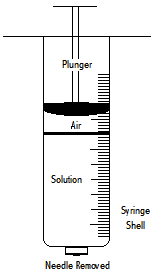
\includegraphics[scale=0.8]{img/syringe.png}
\caption{Measuring volume with a syringe}
\end{center}
\end{figure}

Hazards and Safety: Remove the needle from the syringe. Never use syringes with the needles. Never provide needles to the students.

\subsection*{Squirt Bottle}
Tools Required: Hammer and nail to make hole in lid
Materials Required: Empty bottle, biro casing, IV tubing, super glue.

\begin{figure}[h]
\begin{center}
\def\svgwidth{50pt}
\input{./img/squirt-bottle.pdf_tex}
\caption{Squirt Bottle}
\end{center}
\end{figure}

\subsection*{Test tube}
Tools Required: flame\\
Materials Required: 10 mL plastic syringe\\
Manufacturing Procedure: Remove the plunger from the syringe. Head the nozzle until it starts to melt and then press against a hard surface. If the resulting tube leaks water, heat and press again.
Hazards and Safety: Remove the needle from the syringe. Never use syringes with the needles. Never provide needles to the students.

\subsection*{Test tube holder}
Clothes pin, piece of paper.

\subsection*{Test tube rack}
Tools Required: knife or razor blade\\
Materials Required: cardboard\\
Manufacturing Procedure: Make two parallel folds in the cardboard to elevate the central section. Make "X" cuts in the central section. A test tube can be pushed through these cuts to hold it when not in use.

\begin{figure}[h]
\begin{center}
\def\svgwidth{150pt}
\input{./img/test-tube-rack.pdf_tex}
\caption{Test Tube Rack}
\end{center}
\end{figure}

\subsection*{Water Baths}
If using a kerosene or charcoal stove, this is just a heated pot (sufuria) of water. If using Motopoa, read the instructions in the section on Heat Sources.
